\chapter{CPU Core}

\pulpino supports both the \riscv \rvcore and the \riscv \zerocore. The two
cores have the same external interfaces and are thus plug-compatible.
Figure \ref{fig:riscy_core} and \ref{fig:zero_core} show the two cores
architectures.

The core use a very simple data and instruction interface to talk to data and
instruction memories. To interface with AXI, a core2axi protocol converter is
instantiated in \pulpino.

For debugging purposes, all core registers have been memory mapped which allows
to them to be accessed over the AXI bus. The debug unit inside the core handles
the request over this bus and reads/sets the core registers and/or halts the core.

The core supports performance counters. Those are mainly used for counting core
internal events like stalls, but it is possible to count core-external events
as well. For this purpose there is the \texttt{ext\_perf\_counters\_i} port where
arbitrary events can be attached. The core then increases its internal
performance counter for this event type every time a logic high is seen on this
port.

\begin{figure}[ht]
  \centering
  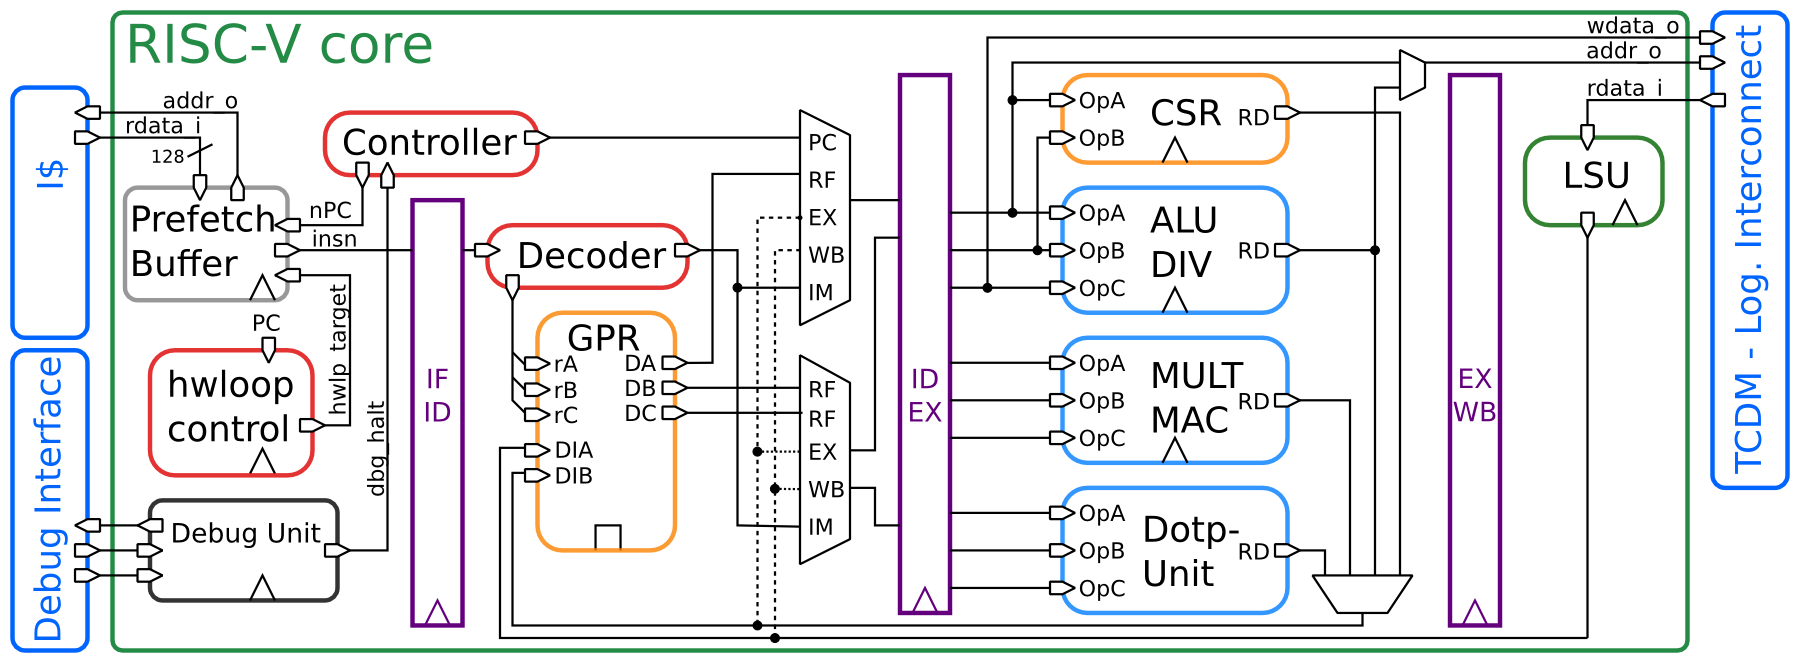
\includegraphics[width=\textwidth]{./figures/riscy_archi.png}
  \caption{RISCY core overview}
  \label{fig:riscy_core}
\end{figure}

\begin{figure}[ht]
  \centering
  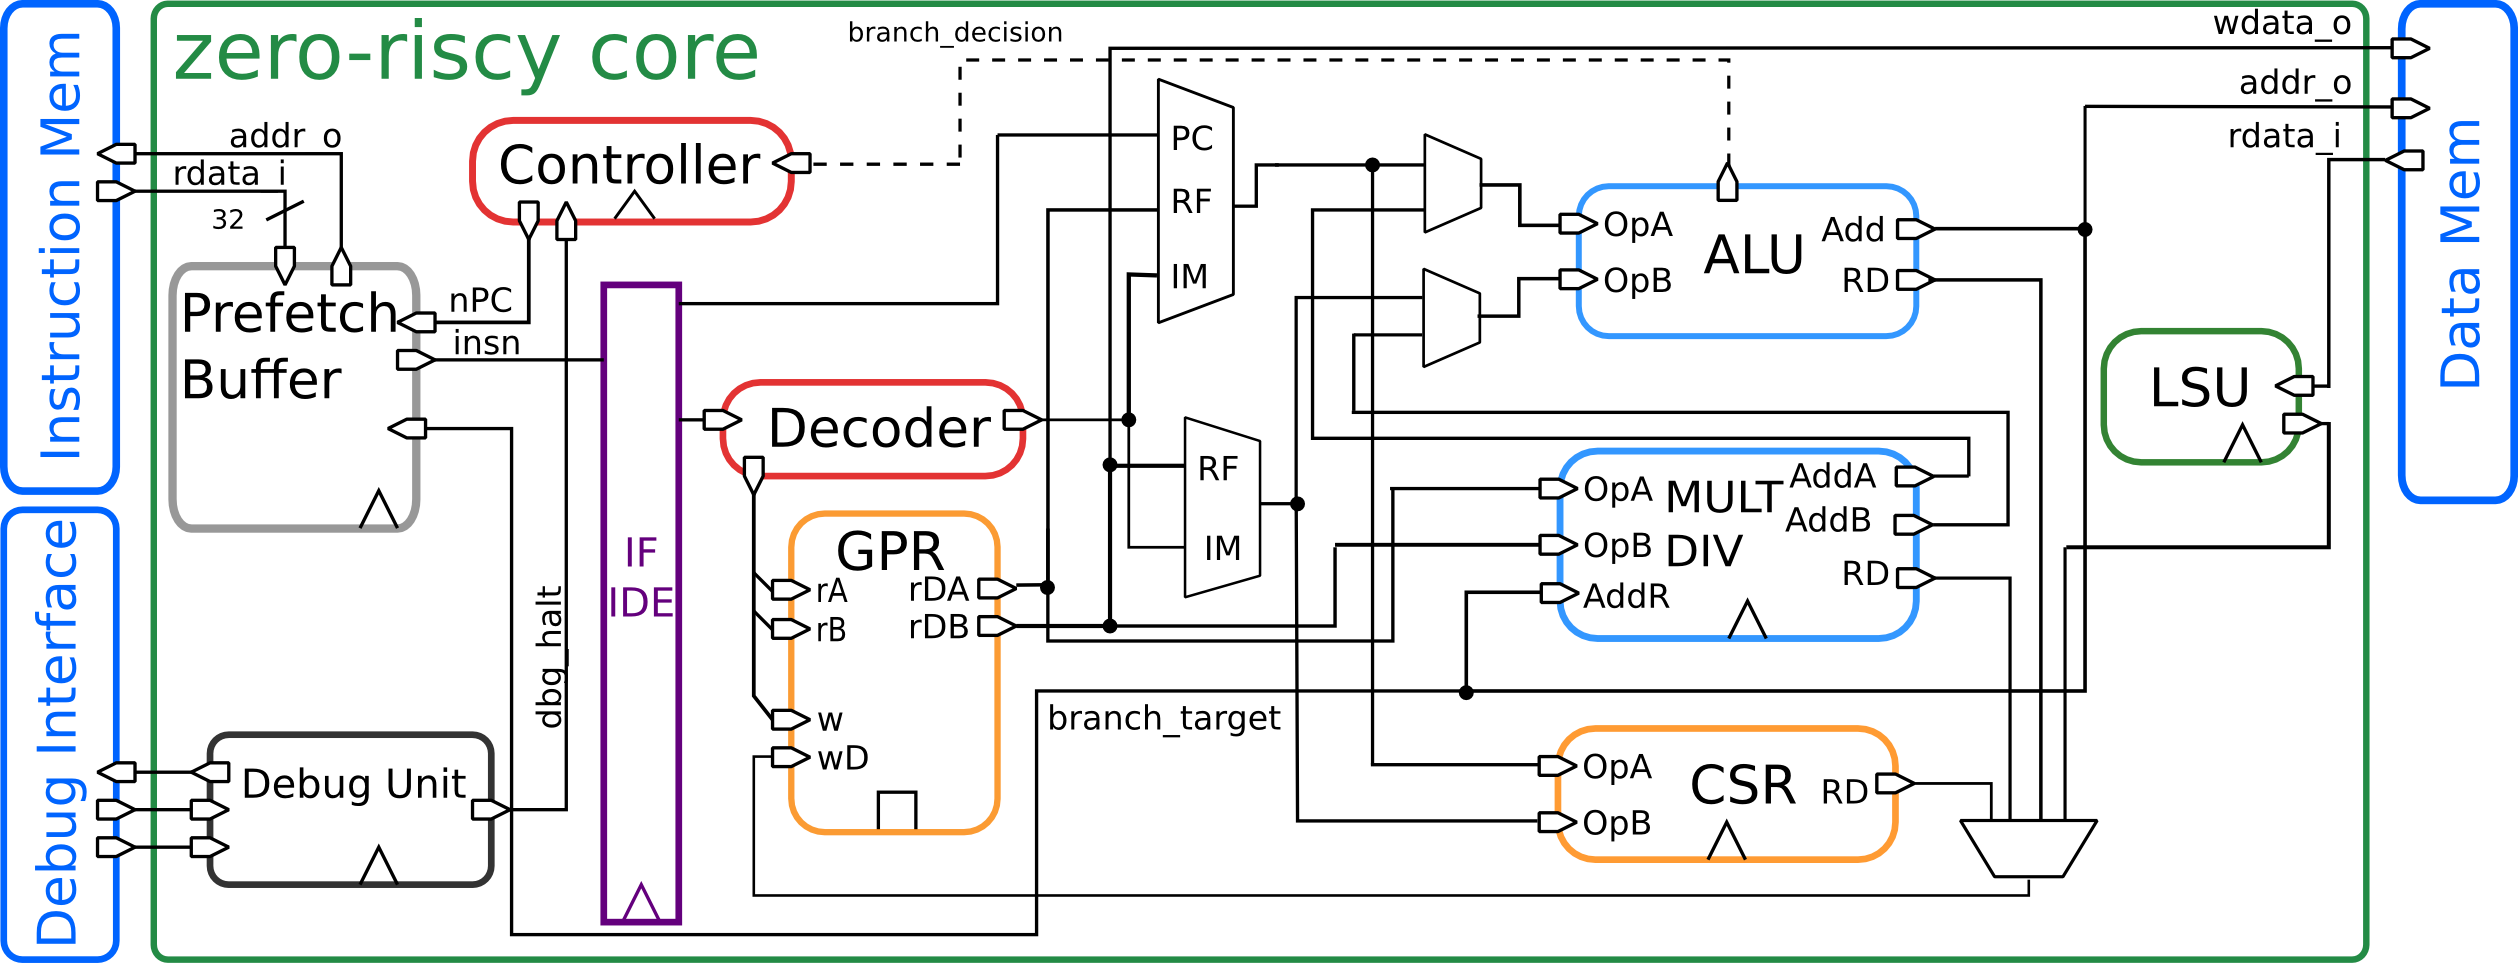
\includegraphics[width=\textwidth]{./figures/zeroriscy_archi.png}
  \caption{zero-riscy core overview}
  \label{fig:zero_core}
\end{figure}
